\documentclass[12pt,a4paper]{article}
\usepackage{graphicx}
\usepackage{amsmath, amssymb, geometry, fancyhdr, cite}
\geometry{margin=2.5cm}
\renewcommand\citeleft{}  % no opening or closing brackets
\renewcommand\citeright{}
\usepackage[colorlinks,citecolor=blue]{hyperref}
\usepackage{xepersian}
\defpersianfont\Vazir[Scale=1]{Vazirmatn}
\settextfont{Vazirmatn}

% Fix header height warning
\setlength{\headheight}{14.49998pt}
\addtolength{\topmargin}{-2.49998pt}

\pagestyle{fancy}
\fancyhf{}
\fancyhead[L]{\lr{MultiModal Agentic RAG}}
\fancyhead[R]{صفحه \thepage}
\fancyfoot[C]{سال ۱۴۰۴}


\setcounter{secnumdepth}{5}
\setcounter{tocdepth}{5}

% Custom command for LTR sections
\newcommand{\LTRSection}[1]{%
    \LTR\section{\textsf{#1}}
}

\begin{document}

% ------- Title Page -------
\thispagestyle{empty}
\begin{center}
    \vspace*{2cm}
    \Huge{دانشگاه فردوسی مشهد} \\[0.5cm]
    \Large{دانشکده علوم ریاضی} \\[2cm]
    \Huge{\LTR\textbf{MultiModal Agentic RAG}} \\[2cm]
    \Large{
        \textbf{درس:} پروژه کارشناسی \\
        \textbf{استاد درس:} دکتر جلال‌الدّین نصیری
    } \\[2cm]
    \Large{
        \textbf{دانشجو:} علی محمودجانلو
    } \\[3cm]
    \Large{سال ۱۴۰۴}
\end{center}

\newpage

% ------- Content Page -------
\thispagestyle{empty}
\hypersetup{linkcolor=blue}
\tableofcontents
\newpage

% ------- Content -------

% Persian Introduction Section
% 
% This section introduces the MultiModal RAG project and the chosen medical textbook

\section{مقدمه}
با رشد روزافزون حجم اطلاعات پزشکی و انتشار مستندات تخصصی در قالب‌های مختلف، دسترسی سریع و دقیق به دانش مورد نیاز در این حوزه به چالشی اساسی تبدیل شده است. کتاب‌های پزشکی تخصصی معمولاً شامل محتوای پیچیده و چندوجهی هستند که ترکیبی از متن، جداول، نمودارها و تصاویر تشخیصی را در بر می‌گیرند. استخراج و بازیابی اطلاعات از این منابع به روش‌های سنتی زمان‌بر و غیرکارآمد است.

در این پروژه، یک سامانه بازیابی اطلاعات چندوجهی مبتنی بر هوش مصنوعی توسعه یافته است که قادر به پردازش هوشمند اسناد پزشکی غیرساختاریافته و ایجاد پایگاه دانش جامع برای پاسخگویی به پرسش‌های تخصصی است. این سامانه از تکنیک‌های پیشرفته پردازش زبان طبیعی، بینایی ماشین و بازیابی تقویت‌شده با تولید \lr{(Retrieval-Augmented Generation - RAG)} بهره می‌برد.

\subsection{منبع داده}
برای ارزیابی و آزمایش سامانه، کتاب \lr{Oxford Textbook of Medicine, 6th Edition} به عنوان منبع اصلی داده انتخاب شده است. این کتاب یکی از معتبرترین و جامع‌ترین مراجع پزشکی در سطح جهان است که توسط انتشارات دانشگاه آکسفورد منتشر شده و شامل چهار جلد و سی بخش تخصصی می‌باشد.

\begin{figure}[h]
    \centering
    
\includegraphics[width=0.5\textwidth]{oxford_cover.jpg}
    \caption{جلد کتاب \lr{Oxford Textbook of Medicine, 6th Edition}}
    \label{fig:oxford_cover}
\end{figure}

\noindent
در این پروژه، جلد دوم این مجموعه که شامل بخش‌های ۱۰ تا ۱۵ است، مورد پردازش قرار گرفته است. این جلد حاوی ۱۸۷۳ صفحه غیرساختاریافته از محتوای پزشکی تخصصی است که طیف وسیعی از موضوعات را پوشش می‌دهد.

\subsection{ویژگی‌های محتوای منبع}
محتوای این جلد دارای ویژگی‌های زیر است که پردازش آن را به چالشی فنی تبدیل می‌کند:

\begin{itemize}
    \item \textbf{ساختار سلسله‌مراتبی پیچیده:} محتوا دارای سطوح متعدد سرفصل، زیربخش و پاراگراف‌های مرتبط است که حفظ این ساختار برای درک صحیح مطالب ضروری است.
    
    \item \textbf{جداول اطلاعاتی متنوع:} صفحات حاوی جداول پیچیده با داده‌های بالینی، آماری و تشخیصی هستند که نیاز به استخراج دقیق و حفظ ساختار دارند.
    
    \item \textbf{محتوای بصری تخصصی:} تصاویر تشخیصی، نمودارها و دیاگرام‌های پزشکی که اطلاعات حیاتی را به صورت بصری منتقل می‌کنند و نیاز به تحلیل هوشمند دارند.
    
    \item \textbf{اصطلاحات تخصصی پزشکی:} استفاده گسترده از واژگان تخصصی، اختصارات و نام‌گذاری‌های علمی که نیاز به پردازش دقیق دارند.
    
    \item \textbf{پیوستگی محتوایی:} ارتباط منطقی بین بخش‌های مختلف که حفظ آن برای درک کامل موضوعات الزامی است.
\end{itemize}

\subsection{اهداف پروژه}
اهداف اصلی این پروژه عبارتند از:

\begin{itemize}
    \item \textbf{تبدیل ساختاریافته:} پردازش اسناد غیرساختاریافته \lr{PDF} و تبدیل آن‌ها به فرمت‌های ساختاریافته با حفظ کامل سلسله‌مراتب و روابط محتوایی.
    
    \item \textbf{پردازش چندوجهی:} استخراج و تحلیل هوشمند متن، جداول و محتوای بصری به صورت یکپارچه.
    
    \item \textbf{نمایه‌سازی هوشمند:} ایجاد پایگاه داده قابل جستجو با حفظ زمینه و ساختار اطلاعات.
    
    \item \textbf{بازیابی دقیق:} پاسخگویی به پرسش‌های تخصصی با استفاده از اطلاعات استخراج‌شده از متن، جداول و تصاویر.
    
    \item \textbf{معماری پاک و قابل توسعه:} طراحی سامانه با رعایت اصول مهندسی نرم‌افزار برای قابلیت نگهداری و توسعه آینده.
\end{itemize}

\subsection{درباره کتاب \lr{Oxford Textbook of Medicine}}
کتاب \lr{Oxford Textbook of Medicine} برجسته‌ترین و معتبرترین کتاب بین‌المللی پزشکی است که به عنوان یک مرجع کلیدی در دفاتر و بخش‌های درمانی پزشکان در سراسر جهان حضور دارد. این کتاب با پوشش بی‌نظیر جنبه‌های علمی و عملکرد بالینی در حوزه طب داخلی و تخصص‌های فرعی آن، همچنین به عنوان منبعی اساسی برای پزشکی قانونی مورد استفاده قرار می‌گیرد.

این اثر جامع، معتبر و بین‌المللی بر ارائه دیدگاه‌های تخصصی و راهنمایی‌های عملی در مدیریت بالینی و پیشگیری از بیماری‌ها تمرکز دارد. بخش‌های مقدماتی این کتاب بر تجربه بیمار، اخلاق پزشکی و تصمیم‌گیری بالینی متمرکز است و فلسفه‌ای انسانی و تفکربرانگیز را ارائه می‌دهد که همواره مشخصه این اثر بوده است. این کتاب به دنبال القای درکی عمیق از نقش پزشکی در جامعه و مشارکت آن در سلامت جمعیت است و از بحث درباره جنبه‌های بحث‌برانگیز پزشکی مدرن طفره نمی‌رود.

\noindent
ویژگی‌های برجسته این کتاب عبارتند از:

\begin{itemize}
    \item \textbf{یکپارچگی علوم پایه و عمل بالینی:} ادغام بی‌نظیر دانش علمی و کاربردهای بالینی در سراسر کتاب، همراه با توضیح پیامدهای تحقیقات برای عملکرد پزشکی.
    
    \item \textbf{پوشش جامع بیماری‌های عفونی:} جامع‌ترین پوشش بیماری‌های عفونی که در هیچ کتاب پزشکی دیگری یافت نمی‌شود.
    
    \item \textbf{موضوعات تخصصی متنوع:} شامل سلول‌های بنیادی و پزشکی بازساختی، نابرابری‌های سلامت، جنبه‌های پزشکی آلودگی و تغییرات اقلیمی، پزشکی سفر و اکسپدیشن، بیوتروریسم و پزشکی قانونی، درد، اختلالات پزشکی در بارداری، تغذیه، و روانپزشکی.
    
    \item \textbf{بخش پزشکی اورژانسی:} طراحی شده برای دسترسی سریع به اطلاعات در مواقع نیاز فوری.
    
    \item \textbf{دسترسی دیجیتال و چاپی:} امکان دسترسی چندگانه بر اساس نیاز و ترجیح کاربران، همراه با به‌روزرسانی‌های منظم در نسخه آنلاین.
    
    \item \textbf{پایگاه مدارک و مراجع پیشرو:} استفاده از جدیدترین یافته‌های تحقیقاتی و شواهد علمی.
\end{itemize}

\noindent
ویرایش ششم این کتاب با بهبودهای قابل توجهی همراه بوده است که در پاسخ به بازخوردهای مستمر کاربران انجام شده است. افزودن بخش‌های خلاصه فصل‌ها برای ارائه دید کلی از محتوا، طراحی جدید برای سهولت خواندن و ناوبری، و همچنین دسترسی رایگان به نسخه آنلاین \lr{Oxford Medicine Online} برای خریداران نسخه چاپی، از جمله این بهبودها هستند.

\noindent
در فصل‌های بعدی، جزئیات معماری سامانه، روش‌های پردازش اسناد، الگوریتم‌های نمایه‌سازی و نتایج ارزیابی به تفصیل ارائه خواهد شد.

\newpage

% بخش معماری پروژه MultiModal RAG
% این فایل جهت ادغام در main.tex طراحی شده است

\section{معماری سیستم}

این پروژه بر اساس الگوی معماری \lr{Clean Architecture} پیاده‌سازی شده است که امکان جداسازی مناسب نگرانی‌ها، مقیاس‌پذیری و نگهداری‌پذیری بالا را فراهم می‌آورد. انتخاب این معماری برای یک سیستم مبتنی بر مدل‌های زبانی بزرگ \lr{(LLM)} که نیازمند انعطاف‌پذیری بالا و قابلیت تست‌پذیری است، از اهمیت ویژه‌ای برخوردار است.

\begin{figure}[h]
    \centering
    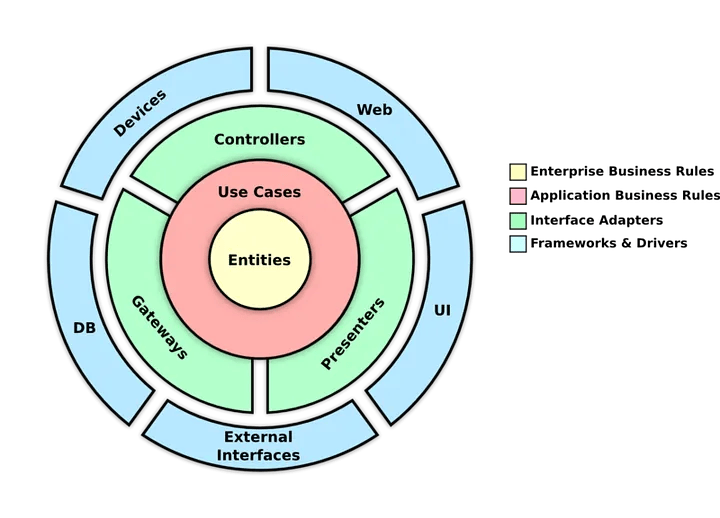
\includegraphics[width=0.8\textwidth]{clean_architecture.png}
    \caption{نمودار معماری \lr{Clean Architecture} و لایه‌های آن}
    \label{fig:clean_architecture}
\end{figure}

\noindent
شکل \ref{fig:clean_architecture} نمودار کلی معماری \lr{Clean} را نشان می‌دهد که در آن جهت وابستگی‌ها از بیرون به درون است و لایه‌های مرکزی از جزئیات پیاده‌سازی مستقل هستند.

\subsection{دلایل انتخاب معماری \lr{Clean}}

انتخاب معماری \lr{Clean} برای این پروژه بر اساس چندین معیار کلیدی صورت گرفته است:

\begin{itemize}    
    \item \textbf{قابلیت تست‌پذیری:} با جداسازی لایه‌های مختلف و استفاده از تزریق وابستگی \lr{(Dependency Injection)}، امکان نوشتن تست‌های واحد و یکپارچه با پوشش بالا میسر می‌شود.
    
    \item \textbf{انعطاف‌پذیری در تعویض ارائه‌دهندگان \lr{LLM}:} سیستم طراحی شده به گونه‌ای است که تغییر یا افزودن ارائه‌دهندگان مختلف \lr{LLM} (مانند \lr{OpenAI}، \lr{Cohere}، یا مدل‌های متن‌باز) بدون تغییر در منطق اصلی امکان‌پذیر است.
    
    \item \textbf{مقیاس‌پذیری:} ساختار لایه‌بندی شده امکان توسعه و گسترش سیستم را در آینده تسهیل می‌کند.
\end{itemize}

\subsection{لایه‌های معماری}

معماری این سیستم شامل چهار لایه اصلی است که هر کدام مسئولیت‌های مشخصی دارند و قانون وابستگی \lr{(Dependency Rule)} در آن‌ها رعایت می‌شود.

\subsubsection{لایه موجودیت‌ها \lr{(Entities)}}

این لایه، قلب سیستم را تشکیل می‌دهد و شامل \lr{enterprise business rules} است که مستقل از هرگونه جزئیات پیاده‌سازی خارجی هستند.

\noindent
\textbf{مسئولیت‌های این لایه:}
\begin{itemize}
    \item تعریف \lr{core data models} با استفاده از \lr{Pydantic}
    \item \lr{Data validation} و اعمال \lr{business rules}
    \item تضمین \lr{type-safety} و \lr{automatic serialization} داده‌ها
\end{itemize}

\noindent
به عنوان مثال، موجودیت \lr{\texttt{DocChunk}} در سیستم ما شامل قوانین کسب‌وکار زیر است:

\begin{itemize}
    \item \textbf{تولید شناسه یکتا:} هر \lr{chunk} باید دارای شناسه‌ای یکتا باشد که بر اساس \lr{\texttt{document\_id}} و \lr{index} تولید می‌شود: \lr{\texttt{\{document\_id\}\_chunk\_\{index\}}}
    
    \item \textbf{اعتبارسنجی بردار \lr{embedding}:} اگر بردار \lr{embedding} موجود باشد، باید از نوع \lr{\texttt{List[float]}} و غیر خالی باشد
    
    \item \textbf{حفظ \lr{metadata} اصلی:} تمام اطلاعات \lr{meta} شامل \lr{schema\_name}، \lr{version} و \lr{doc\_items} باید حفظ شوند
    
    \item \textbf{تبدیل فرمت:} موجودیت باید قابلیت تبدیل دوطرفه به فرمت \lr{Elasticsearch} و \lr{Docling} را داشته باشد
\end{itemize}

\noindent
این قوانین مستقل از جزئیات پیاده‌سازی \lr{database} یا \lr{search engine} تعریف شده‌اند و در صورت تغییر فناوری زیرساخت، دست‌نخورده باقی می‌مانند.


\subsubsection{لایه \lr{(Use Cases)}}

این لایه \lr{application business logic} را در بر می‌گیرد و \lr{workflow} بین \lr{entities} و \lr{interface adapters} را هماهنگ می‌کند.

\noindent
\textbf{مسئولیت‌های کلیدی:}
\begin{itemize}
    \item مدیریت جریان‌های کاری پیچیده با استفاده از \lr{LangGraph}
    \item پیاده‌سازی \lr{RAG (Retrieval-Augmented Generation) pipelines}
    \item تولید و مدیریت \lr{embeddings}
    \item هماهنگی با سرویس‌های خارجی از طریق \lr{interfaces}
\end{itemize}

\noindent
\textbf{\lr{Data Transfer Objects (DTOs)}:}

\lr{DTOs} مدل‌های داده‌ای هستند که به‌طور خاص برای انتقال داده بین لایه‌های مختلف طراحی شده‌اند. این \lr{objects} در فایل \lr{\texttt{usecases/dtos.py}} قرار می‌گیرند و زمانی استفاده می‌شوند که:
\begin{itemize}
    \item \lr{Public APIs} (\lr{REST}، \lr{GraphQL} و غیره) ساخته می‌شود
    \item یکپارچگی با سیستم‌های خارجی با \lr{data models} متفاوت مورد نیاز است
    \item نیاز به \lr{versioning} دقیق و \lr{backward compatibility} وجود دارد
\end{itemize}

\subsubsection{لایه آداپتورهای رابط \lr{(Interface Adapters)}}

این لایه وظیفه تبدیل داده‌ها بین موارد استفاده و دنیای خارج را بر عهده دارد.

\noindent
\textbf{اجزای این لایه شامل:}
\begin{itemize}
    \item \textbf{\lr{Controllers}:} مدیریت \lr{HTTP requests} و \lr{responses}
    \item \textbf{\lr{Presenters}:} قالب‌بندی داده‌ها برای رابط کاربری یا مصرف‌کنندگان \lr{API}
    \item \textbf{\lr{Gateways}:} رابط با سرویس‌های خارجی مانند \lr{databases}، \lr{vector stores} و \lr{third-party APIs}
\end{itemize}

\subsubsection{لایه فریم‌ورک‌ها و درایورها \lr{(Frameworks and Drivers)}}

بیرونی‌ترین لایه سیستم که شامل جزئیات پیاده‌سازی ابزارها و فریم‌ورک‌های خارجی است.

\noindent
\textbf{مثال‌های موجود در این لایه:}
\begin{itemize}
    \item \lr{Web frameworks} (\lr{FastAPI}، \lr{Flask})
    \item \lr{LLM providers} (\lr{OpenAI}، \lr{Cohere}، \lr{open-source models})
    \item \lr{Databases} و \lr{vector stores} (\lr{Elasticsearch}، \lr{Redis}، \lr{Pinecone})
    \item فریم‌ورک‌هایی مانند \lr{LangChain} و \lr{LangGraph}
\end{itemize}

\subsection{اصول طراحی}

\subsubsection{قانون وابستگی \lr{(Dependency Rule)}}

در این معماری، وابستگی‌ها همواره از لایه‌های بیرونی به سمت لایه‌های درونی هستند. این بدان معناست که:

\begin{equation}
\text{\lr{Frameworks/Drivers}} \rightarrow \text{\lr{Interface Adapters}} \rightarrow \text{\lr{Use Cases}} \rightarrow \text{\lr{Entities}}
\end{equation}

\noindent
لایه‌های درونی هیچ‌گونه اطلاعی از لایه‌های بیرونی ندارند و این استقلال امکان تغییر پیاده‌سازی‌های خارجی را بدون تأثیر بر هسته سیستم فراهم می‌آورد.

\subsubsection{اصل وارونگی وابستگی \lr{(Dependency Inversion Principle)}}

برای حفظ قانون وابستگی، از \lr{interfaces} و کلاس‌های انتزاعی استفاده می‌شود. به این ترتیب:

\begin{itemize}
    \item \lr{Interfaces} در لایه‌های هسته (\lr{Use Cases}) تعریف می‌شوند
    \item پیاده‌سازی‌های واقعی در لایه‌های بیرونی (\lr{Interface Adapters} یا \lr{Frameworks}) قرار می‌گیرند
    \item لایه‌های سطح بالا به انتزاع وابسته‌اند، نه به پیاده‌سازی‌های خاص
\end{itemize}

\subsection{سیستم \lr{Dependency Injection}}

برای مدیریت وابستگی‌ها و پیکربندی سیستم، از کتابخانه \lr{\texttt{dependency-injector}} استفاده شده است. این سیستم مزایای زیر را فراهم می‌آورد:

\subsubsection{مزایای \lr{Dependency Injection}}

\begin{itemize}
    \item \textbf{\lr{Centralized configuration}:} تمام تنظیمات و وابستگی‌ها در یک \lr{container} مرکزی مدیریت می‌شوند
    \item \textbf{تسهیل تست:} امکان جایگزینی وابستگی‌های واقعی با \lr{mocks} برای تست‌نویسی
    \item \textbf{مدیریت \lr{singleton}:} کنترل \lr{lifecycle} منابع گران‌قیمت مانند \lr{database connections}
    \item \textbf{انعطاف‌پذیری:} تغییر \lr{configuration} در \lr{runtime} بدون تغییر کد
\end{itemize}

\subsubsection{ساختار \lr{container}}

درخت وابستگی سیستم به صورت زیر سازماندهی شده است:

\begin{verbatim}
ApplicationContainer
├── Configuration (from env/files)
├── LoggerFactory (Singleton)
├── ElasticsearchConfig (Singleton)
├── AsyncElasticsearch (Singleton)
├── ElasticsearchDocumentAdaptor (Singleton)
├── EmbeddingService (Factory)
├── DocumentIndexingUseCase (Factory)
└── DocumentSearchUseCase (Factory)
\end{verbatim}

\noindent
\textbf{انواع \lr{providers}:}
\begin{itemize}
    \item \textbf{\lr{Factory}:} برای ایجاد نمونه جدید در هر بار استفاده
    \item \textbf{\lr{Singleton}:} برای نگهداری یک نمونه واحد
    \item \textbf{\lr{Resource}:} برای مدیریت چرخه حیات اشیاء پیچیده
    \item \textbf{\lr{Configuration}:} برای مدیریت مقادیر پیکربندی
\end{itemize}

\subsection{یکپارچگی با فریم‌ورک‌های \lr{LLM}}

یکی از چالش‌های اصلی این پروژه، یکپارچگی با فریم‌ورک‌های مختلف \lr{LLM} بوده است. معماری طراحی شده این امکان را فراهم می‌آورد که:

\begin{itemize}
    \item از چندین ارائه‌دهنده \lr{LLM} به صورت همزمان استفاده شود
    \item جریان‌های کاری پیچیده با \lr{LangGraph} مدیریت شوند
    \item عملیات \lr{RAG} به صورت ماژولار پیاده‌سازی شوند
    \item تغییر یا ارتقای فریم‌ورک‌ها بدون تغییر منطق اصلی امکان‌پذیر باشد
\end{itemize}

\subsection{استفاده از \lr{Pydantic}}

در لایه موجودیت‌ها، از کتابخانه \lr{Pydantic} برای تعریف \lr{data models} استفاده شده است. این انتخاب به دلایل زیر صورت گرفته است:

\begin{itemize}
    \item \textbf{\lr{Automatic validation}:} داده‌ها به صورت خودکار در زمان ایجاد \lr{object} اعتبارسنجی می‌شوند
    \item \textbf{\lr{Type Safety}:} تضمین صحت \lr{data types} در زمان توسعه
    \item \textbf{\lr{Serialization}:} تبدیل خودکار به \lr{JSON} و سایر فرمت ها
    \item \textbf{\lr{Automatic documentation}:} تولید \lr{schema} برای \lr{APIs}
\end{itemize}

\subsection{مدیریت \lr{Error} و \lr{Logging}}

سیستم دارای یک لایه یکپارچه برای \lr{error handling} و \lr{logging} است که:

\begin{itemize}
    \item از \lr{multi-level logging} پشتیبانی می‌کند
    \item خطاها را به صورت ساختاریافته ثبت می‌کند
    \item امکان \lr{request tracing} را فراهم می‌آورد
    \item با سیستم‌های \lr{monitoring} خارجی قابل یکپارچگی است
\end{itemize}

\noindent
سیستم \lr{logging} پیاده‌سازی شده در این پروژه، از قابلیت \lr{automatic rotation} و مدیریت \lr{log levels} مختلف برخوردار است. شکل \ref{fig:logging_example} نمونه‌ای از خروجی سیستم \lr{logging} را نشان می‌دهد که شامل \lr{timestamp}، نام \lr{module}، \lr{log level}، و \lr{message} مربوطه است.

\begin{figure}[h]
    \centering
    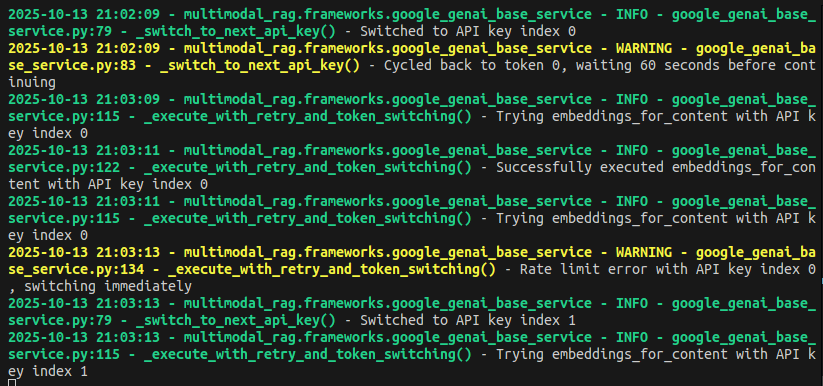
\includegraphics[width=\textwidth]{logging_example.png}
    \caption{نمونه \lr{output} سیستم \lr{logging}}
    \label{fig:logging_example}
\end{figure}

\subsection{مزایای معماری اتخاذ شده}

پیاده‌سازی معماری \lr{Clean} در این پروژه مزایای زیر را به همراه داشته است:

\begin{enumerate}
    \item \textbf{\lr{High Maintainability}:} جداسازی واضح مسئولیت‌ها، درک و نگهداری کد را آسان می‌کند
    
    \item \textbf{\lr{Testability}:} هر لایه به صورت مستقل قابل تست است و نیازی به راه‌اندازی کل سیستم نیست
    
    \item \textbf{\lr{Flexibility}:} تغییر یا جایگزینی اجزای سیستم بدون تأثیر بر سایر بخش‌ها امکان‌پذیر است

    \item \textbf{\lr{Scalability}:} افزودن قابلیت‌های جدید به دلیل ساختار ماژولار، آسان‌تر است

    \item \textbf{\lr{Technology Independence}:} عدم وابستگی به فریم‌ورک‌ها و کتابخانه‌های خاص

    \item \textbf{\lr{Better Team Collaboration}:} اعضای تیم می‌توانند به صورت موازی بر روی لایه‌های مختلف کار کنند
\end{enumerate}

\subsection{چالش‌ها و راه‌حل‌ها}

در طول پیاده‌سازی این معماری، چالش‌هایی نیز وجود داشت که به شرح زیر برطرف شدند:

\begin{itemize}
    \item \textbf{\lr{Initial Complexity}:} راه‌اندازی اولیه سیستم زمان‌بر بود، اما این سرمایه‌گذاری در بلندمدت به صرفه بوده است
    
    \item \textbf{\lr{Circular Dependencies}:} با طراحی دقیق \lr{interfaces} و استفاده از \lr{dependency inversion} از آن جلوگیری شد
    
    \item \textbf{\lr{Performance}:} استفاده از \lr{singleton pattern} برای \lr{expensive resources} و \lr{caching} مناسب، مسائل \lr{performance} را برطرف کرد
    
    \item \textbf{\lr{Learning Curve}:} مستندسازی جامع و مثال‌های کاربردی، فهم معماری را برای توسعه‌دهندگان جدید تسهیل کرد
\end{itemize}

\newpage

\section{نتیجه‌گیری معماری}

معماری \lr{Clean} برای این پروژه \lr{MultiModal RAG}، بستری مناسب برای توسعه یک سیستم \lr{scalable}، \lr{maintainable} و \lr{flexible} فراهم آورده است. جداسازی واضح لایه‌ها، استفاده از \lr{dependency injection}، و رعایت اصول \lr{SOLID}، امکان توسعه پایدار و با کیفیت این سیستم را در بلندمدت تضمین می‌کند. این رویکرد معماری به‌ویژه برای سیستم‌های مبتنی بر \lr{LLM} که نیازمند \lr{flexibility} بالا در تعویض \lr{providers} و \lr{models} هستند، مناسب است.

\newpage

% بخش Docling - ابزار پردازش اسناد چندوجهی

\section{پردازش و نمایه‌سازی اسناد با \lr{Docling}}

\subsection{معرفی \lr{Docling}}
\lr{Docling} یک کتابخانه منبع‌باز پیشرفته برای پردازش و تبدیل اسناد ساختارنیافته به فرمت‌های قابل استفاده در سیستم‌های بازیابی اطلاعات است. این ابزار توسط تیم تحقیقاتی \lr{IBM} توسعه یافته و به‌صورت رایگان در دسترس جامعه علمی قرار گرفته است. \lr{Docling} با استفاده از مدل‌های یادگیری عمیق پیشرفته، قادر به تشخیص ساختار سلسله‌مراتبی اسناد، استخراج جداول پیچیده، و پردازش محتوای چندوجهی شامل متن، تصاویر و نمودارها می‌باشد.

\noindent
ویژگی‌های کلیدی \lr{Docling} عبارتند از:
\begin{itemize}
    \item \textbf{تشخیص ساختار سلسله‌مراتبی:} شناسایی خودکار عناوین، زیرعناوین، پاراگراف‌ها، و بخش‌های مختلف سند
    \item \textbf{استخراج دقیق جداول:} تبدیل جداول پیچیده با سلول‌های ادغام‌شده به فرمت ساختاریافته
    \item \textbf{پشتیبانی از محتوای چندوجهی:} پردازش همزمان متن، تصاویر، نمودارها و فرمول‌های ریاضی
    \item \textbf{خروجی استاندارد:} تولید فایل‌های \lr{JSON} ، \lr{YAML} و \lr{Markdown} با حفظ روابط والد-فرزندی بین عناصر
    \item \textbf{تکه‌سازی هوشمند:} ترکیب عناصر مرتبط در تکه‌های معنادار با رعایت محدودیت‌های طول توکن
\end{itemize}

\begin{figure}[!htbp]
    \centering
    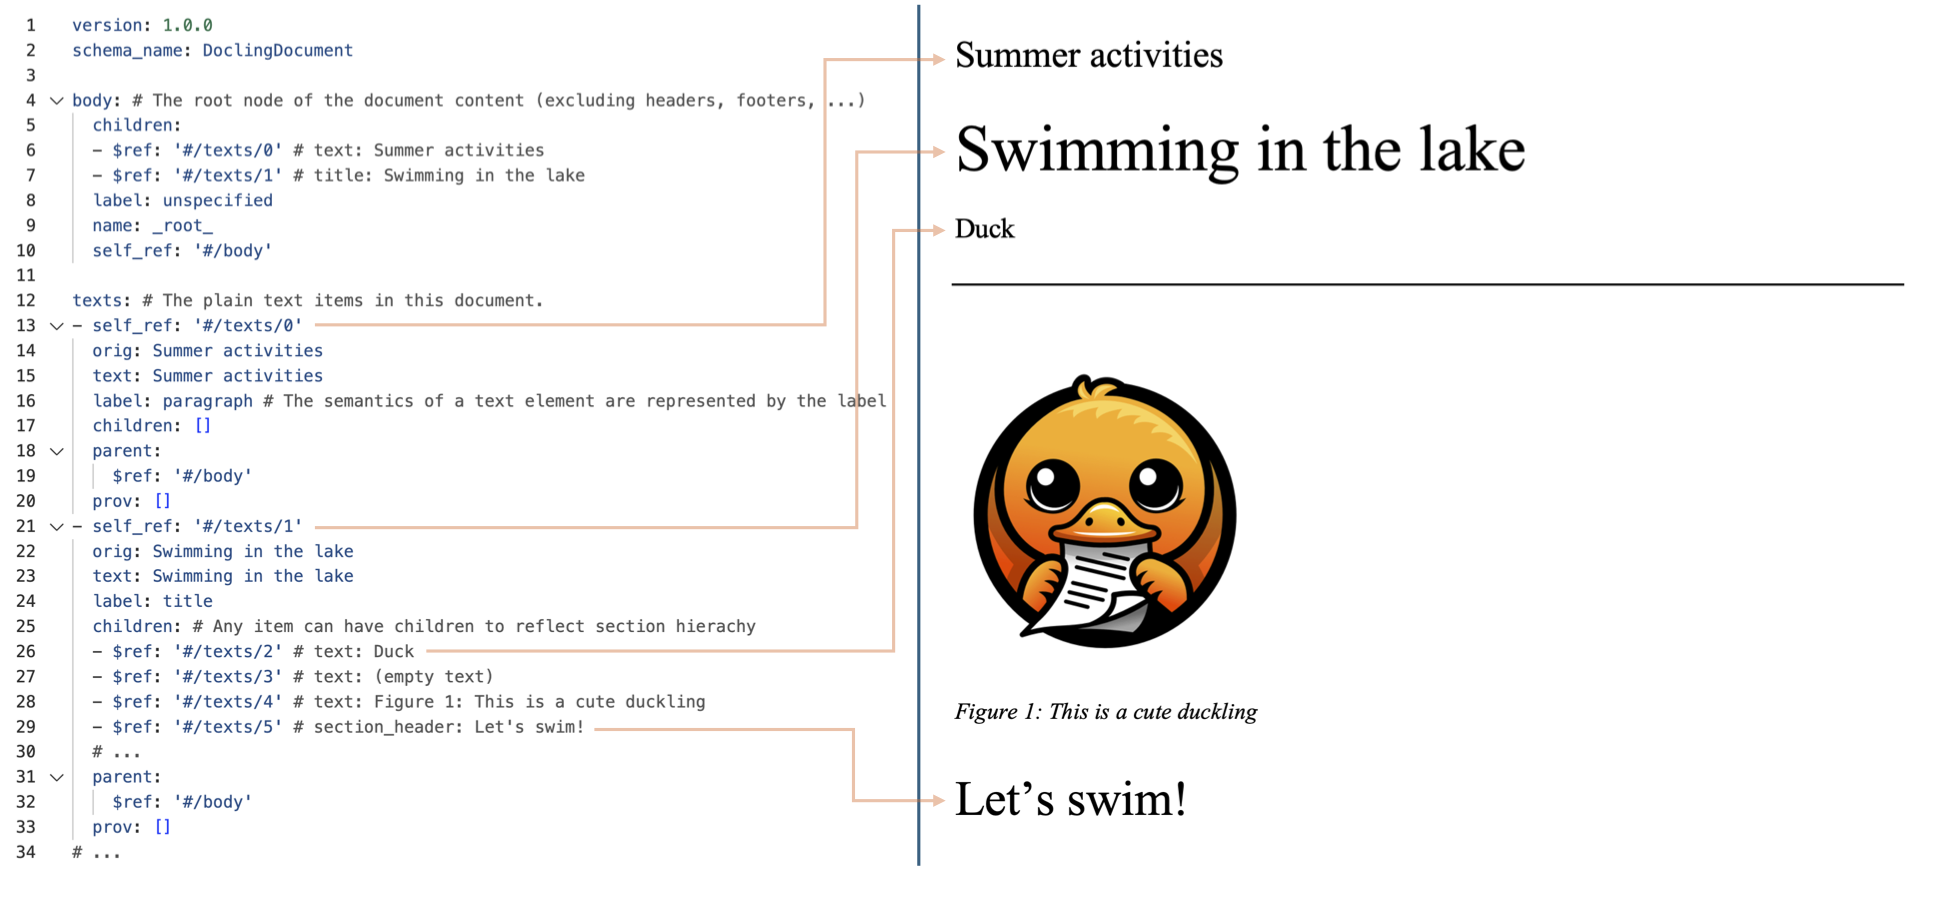
\includegraphics[width=0.95\textwidth]{docling_doc_hierarchy_1.png}
    \caption{نمونه‌ای از ساختار \lr{DoclingDocument}. سمت راست صفحه‌ای با عناوین، تصویر، زیرنویس و پاراگراف‌ها را نشان می‌دهد. سمت چپ درخت سند را نمایش می‌دهد که در آن هر عنصر با برچسب و اشاره‌گر خود در ساختار سلسله‌مراتبی قرار گرفته است.}
    \label{fig:docling_structure}
\end{figure}

\begin{figure}[!htbp]
    \centering
    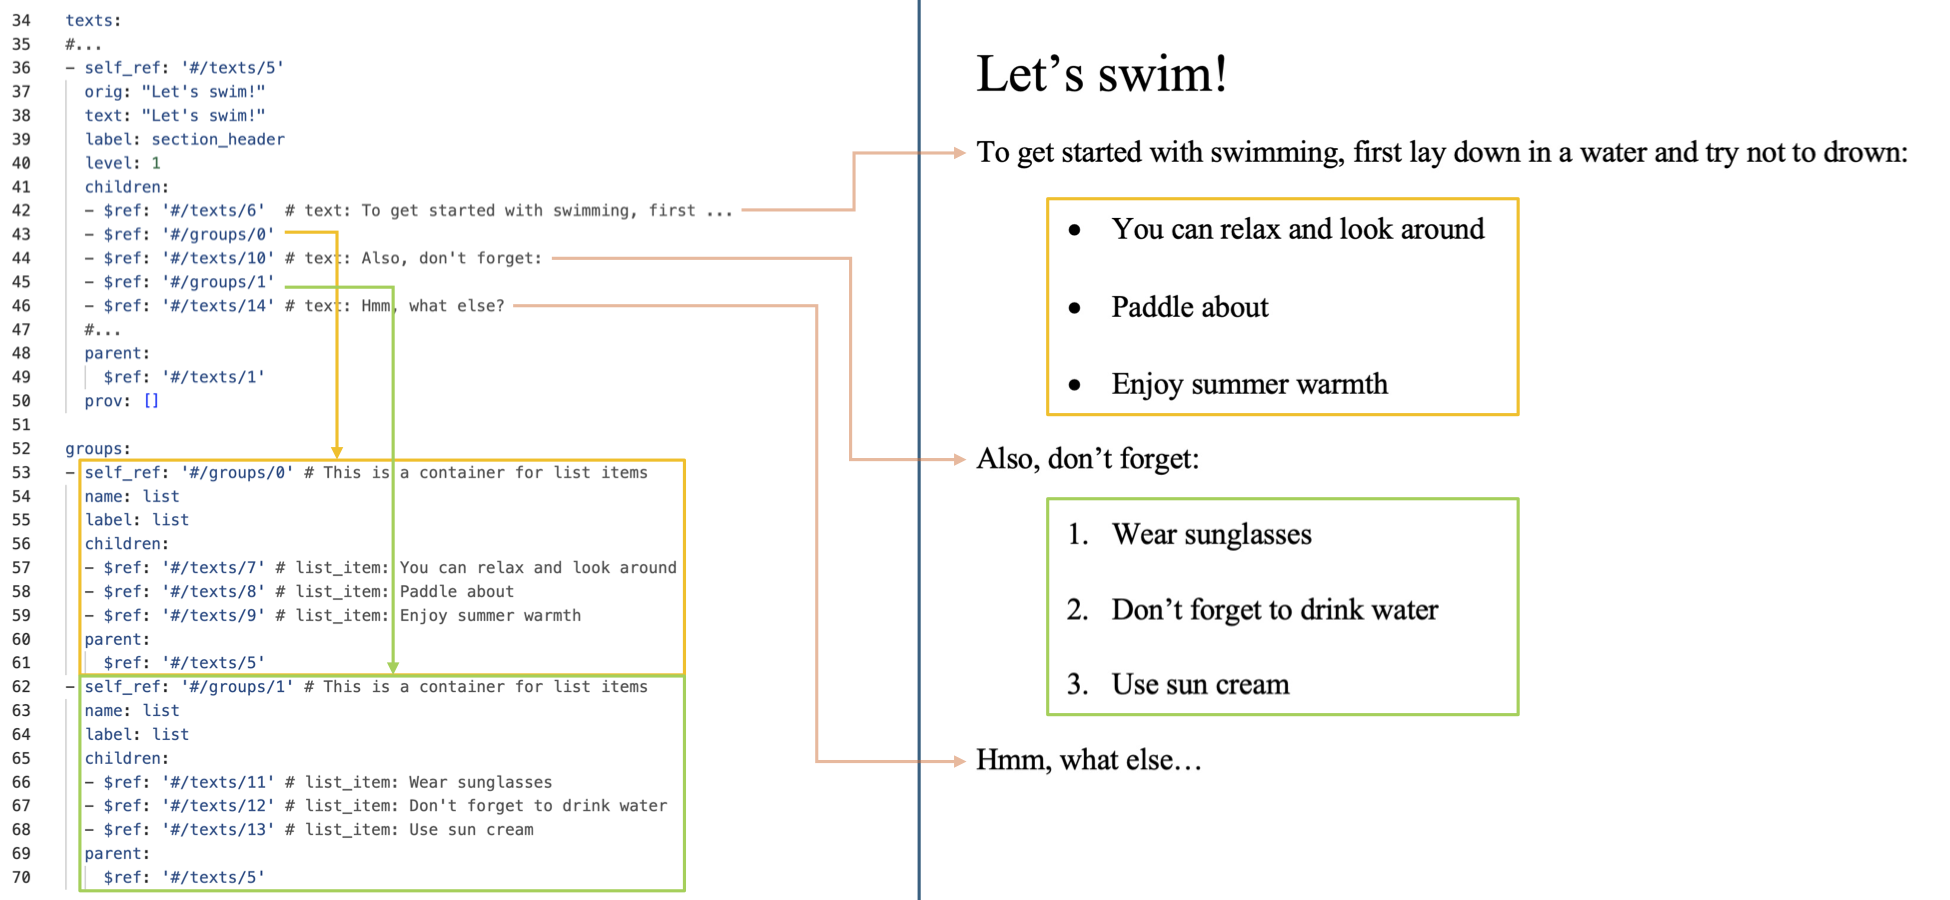
\includegraphics[width=0.95\textwidth]{docling_doc_hierarchy_2.png}
    \caption{فهرست‌های تو در تو و گروه‌ها در \lr{DoclingDocument}. سمت راست دو فهرست (یکی نقطه‌ای و دیگری شماره‌دار) را نشان می‌دهد. سمت چپ نشان می‌دهد که هر فهرست در یک کانتینر گروهی قرار می‌گیرد و عناصر آن به‌عنوان فرزند اضافه می‌شوند.}
    \label{fig:docling_groups}
\end{figure}

\subsection{دلایل انتخاب \lr{Docling}}
انتخاب \lr{Docling} به‌عنوان ابزار اصلی نمایه‌سازی کتاب پزشکی در این پروژه بر اساس ارزیابی دقیق نیازمندی‌های سیستم و مقایسه با ابزارهای موجود انجام شده است. در ادامه مهم‌ترین دلایل این انتخاب شرح داده می‌شود.

\subsubsection{پردازش اسناد پزشکی پیچیده}
اسناد پزشکی از پیچیده‌ترین انواع محتوای علمی هستند که شامل ترکیبی از متن تخصصی، جداول آماری، تصاویر تشخیصی، نمودارهای آناتومیکی و فرمول‌های دارویی می‌باشند. \lr{Docling} با معماری پردازشی چندمرحله‌ای خود، قادر به تشخیص و استخراج دقیق این عناصر متنوع است. برخلاف ابزارهای سنتی که صفحات را به‌صورت یک‌پارچه پردازش می‌کنند، \lr{Docling} از یک خط‌لوله مرحله‌ای استفاده می‌کند که در آن هر نوع محتوا با مدل تخصصی خود پردازش می‌شود.

\subsubsection{معماری مبتنی بر مدل‌های تخصصی}
یکی از برتری‌های اصلی \lr{Docling} نسبت به روش‌های مبتنی بر مدل‌های زبانی بزرگ چندوجهی \lr{(Vision Language Models)} این است که به‌جای استفاده از یک مدل عمومی برای تمام وظایف، از مدل‌های تخصصی برای هر بخش استفاده می‌کند:

\begin{itemize}
    \item \textbf{مدل تحلیل چیدمان (\lr{Layout Analysis}):} \lr{Docling} از مدل \lr{Heron} مبتنی بر معماری \lr{RT-DETR} با پشتوانه \lr{ResNet-50} استفاده می‌کند که روی مجموعه داده \lr{DocLayNet} شامل بیش از ۸۰ هزار صفحه برچسب‌گذاری شده آموزش دیده است. این مدل قادر به تشخیص ۱۷ کلاس مختلف شامل عنوان، متن، فهرست، جدول، تصویر، عنوان بخش، فرمول، زیرنویس و سایر عناصر است. دقت این مدل بر روی مجموعه داده استاندارد \lr{DocLayNet} به ۷۸ درصد \lr{mAP} می‌رسد (شکل \ref{fig:doclaynet_labels}).
\end{itemize}

\begin{figure}[!htbp]
    \centering
    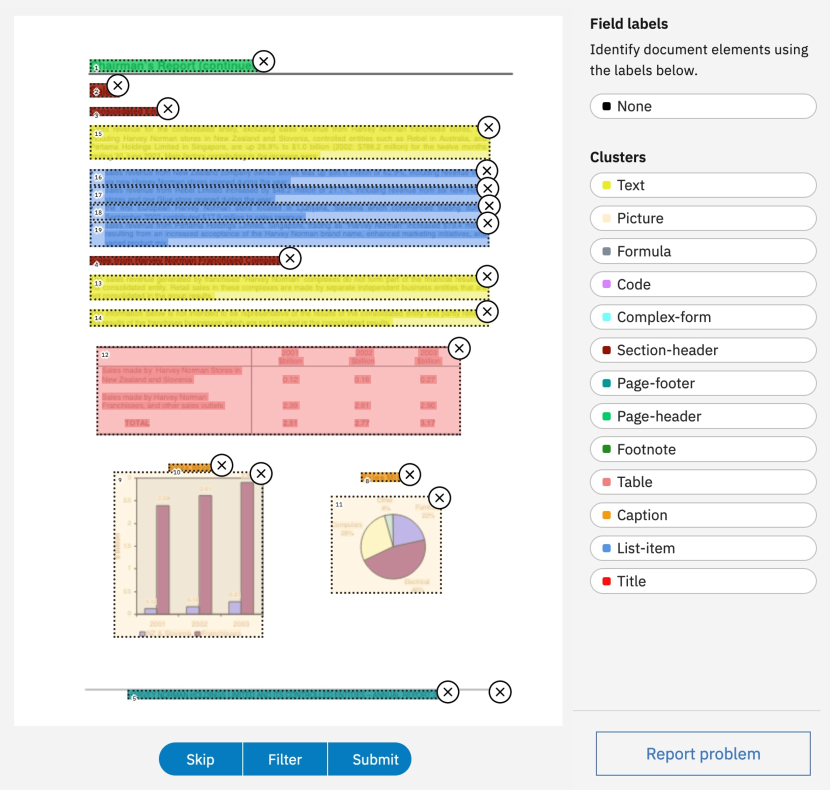
\includegraphics[width=0.65\textwidth]{doclaynet.png}
    \caption{نمونه‌ای از برچسب‌گذاری عناصر مختلف سند در مجموعه داده \lr{DocLayNet}. این تصویر نشان می‌دهد که چگونه هر عنصر صفحه (متن، عنوان، جدول، تصویر، فهرست و غیره) با کلاس‌های مختلف شناسایی و برچسب‌گذاری می‌شود. این برچسب‌های دقیق انسانی پایه آموزش مدل \lr{Heron} را تشکیل می‌دهند.}
    \label{fig:doclaynet_labels}
\end{figure}

\begin{itemize}
    \item \textbf{مدل استخراج ساختار جداول (\lr{TableFormer}):} برای پردازش جداول پیچیده، \lr{Docling} از مدل \lr{TableFormer} استفاده می‌کند که یک معماری ترنسفورمر مبتنی بر بینایی است. این مدل روی مجموعه داده‌های بزرگ شامل \lr{PubTabNet} (بیش از ۲۲۷ هزار جدول) آموزش دیده و قادر به تشخیص سطرها، ستون‌ها، سلول‌های ادغام‌شده، و ساختارهای پیچیده جداول است. خروجی این مدل شامل توالی توکن‌های \lr{HTML} و مختصات مرزی هر سلول است که سپس با متن اصلی \lr{PDF} تطبیق داده می‌شود (شکل \ref{fig:table_extraction}).
\end{itemize}

\begin{figure}[!htbp]
    \centering
    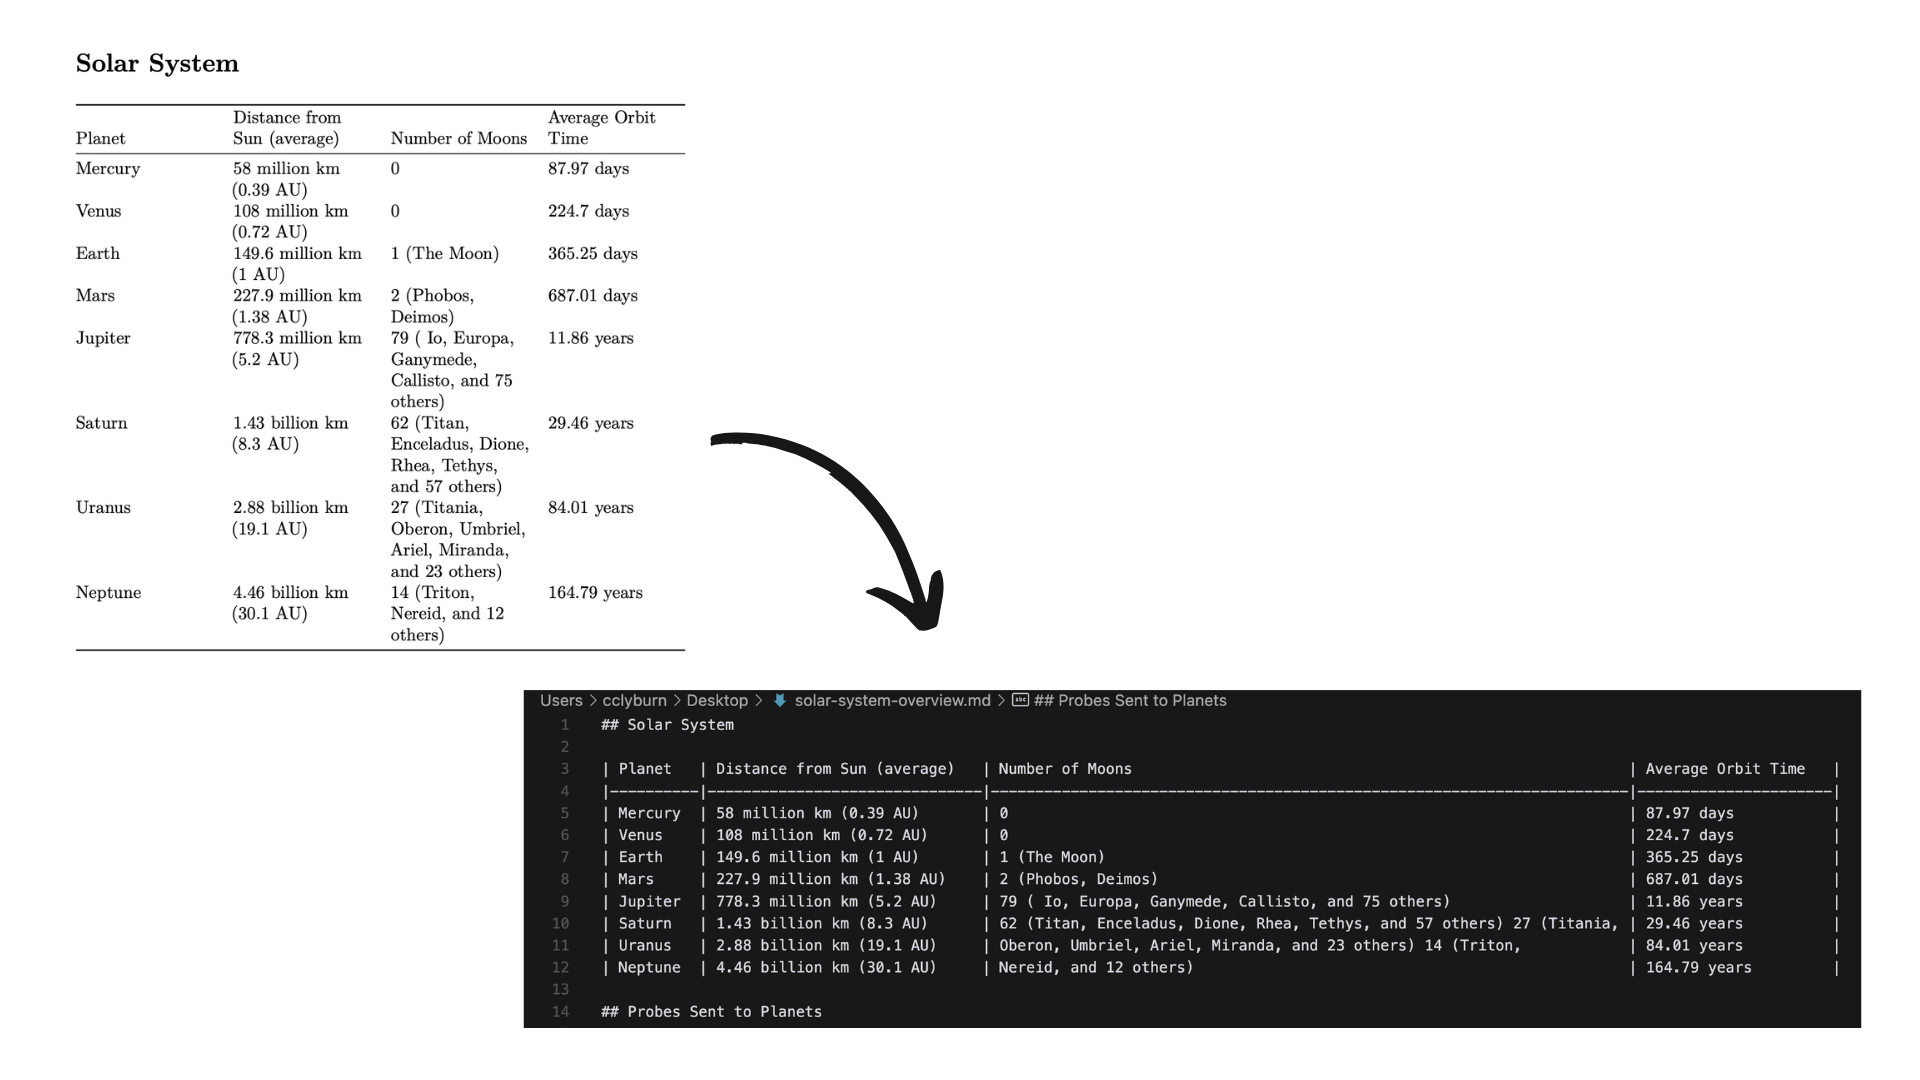
\includegraphics[width=0.85\textwidth]{docling_md_2.png}
    \caption{مثالی از استخراج دقیق جدول توسط \lr{TableFormer}. بالا: جدول اصلی منظم شامل اطلاعات سیارات منظومه شمسی. پایین: جدول استخراج شده در فرمت \lr{Markdown} که ساختار دقیق ستون‌ها و سطرها حفظ شده است.}
    \label{fig:table_extraction}
\end{figure}

\begin{itemize}
    \item \textbf{مدل توصیف تصاویر (\lr{Picture Description Model}):} یکی از چالش‌های مهم در پردازش کتاب‌های پزشکی، تولید توصیفات دقیق و جامع از تصاویر پیچیده پزشکی است. مدل پیش‌فرض \lr{Docling} برای این منظور \lr{SmolVLM} با حدود ۲۵۶ میلیون پارامتر است. با وجود سبک بودن این مدل، عملکرد آن در توصیف تصاویر پیچیده و نموداری پزشکی مطلوب نبود. در مرحله بعد، از مدل \lr{Granite-3.1 Vision} شرکت \lr{IBM} با ۲ میلیارد پارامتر استفاده شد که نتایج بهتری ارائه داد، اما به دلیل مشکل نشت حافظه \lr{(Memory Leak)} در \lr{Docling}، اجرای پایدار آن در محیط \lr{Google Colab} با \lr{GPU T4} امکان‌پذیر نبود. در نهایت، برای دستیابی به بهترین کیفیت توصیف، از \lr{API} رایگان مدل \lr{Gemini 2.5-Flash} شرکت \lr{Google} استفاده شد. برای مدیریت محدودیت‌های نرخ درخواست، یک سیستم تعویض خودکار بین توکن‌های مختلف پیاده‌سازی شد تا در صورت برخورد به خطای محدودیت نرخ با یک توکن، به‌طور خودکار از توکن دیگری استفاده شود و پردازش بدون وقفه ادامه یابد (شکل \ref{fig:picture_description}).
\end{itemize}

\begin{figure}[!htbp]
    \centering
    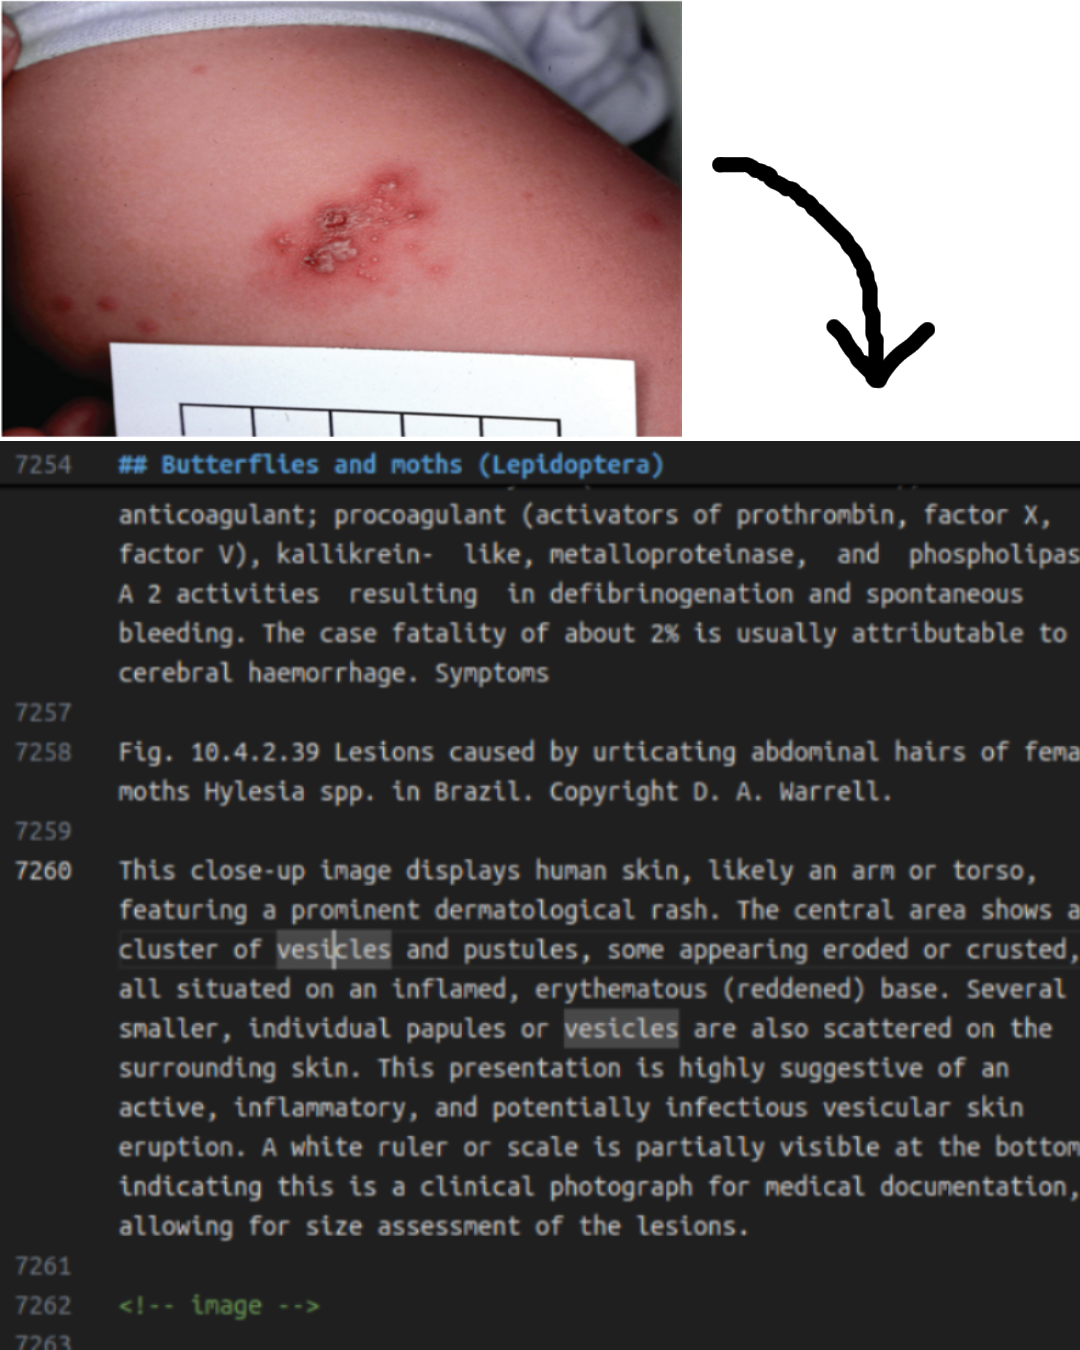
\includegraphics[width=0.95\textwidth]{picture_description.png}
    \caption{نمونه‌ای از خروجی مدل توصیف تصویر \lr{Gemini 2.5-Flash} برای یک تصویر پزشکی پیچیده. تصویر بالا یک ضایعه پوستی ناشی از تماس با موی بید برزیلی را نشان می‌دهد که شامل تاول‌ها و پاپول‌های قرمز روی پوست انسان است. مدل \lr{Gemini} توانسته است جزئیات کامل تصویر شامل نوع ضایعه، موقعیت آناتومیکی، و ویژگی‌های بالینی را به‌طور دقیق توصیف کند، که نشان‌دهنده برتری آن نسبت به مدل‌های سبک‌تر مانند \lr{SmolVLM} در پردازش تصاویر پزشکی پیچیده است.}
    \label{fig:picture_description}
\end{figure}

\begin{itemize}
    \item \textbf{موتور تشخیص نوشتار (\lr{OCR}):} برای پردازش محتوای اسکن‌شده یا تصویری، \lr{Docling} از \lr{EasyOCR} استفاده می‌کند که یک کتابخانه یادگیری عمیق مبتنی بر \lr{PyTorch} است. این موتور از مدل \lr{CRAFT} برای تشخیص مناطق متنی و مدل \lr{CRNN} برای خواندن کاراکترها استفاده می‌کند. \lr{Docling} صفحات را با وضوح ۲۱۶ \lr{DPI} رندر کرده و برای دستیابی به دقت بالا در تشخیص فونت‌های کوچک، از این موتور بهره می‌برد.
\end{itemize}

\noindent
این معماری متخصص‌محور باعث می‌شود دقت پردازش در مقایسه با مدل‌های عمومی چندوجهی به‌طور قابل توجهی افزایش یابد، زیرا هر مدل فقط بر روی یک وظیفه خاص تمرکز دارد و برای آن بهینه‌سازی شده است.

\subsubsection{حفظ ساختار سلسله‌مراتبی و روابط معنایی}
یکی از چالش‌های اساسی در پردازش اسناد پزشکی، حفظ روابط سلسله‌مراتبی بین عناصر مختلف است. کتاب‌های پزشکی دارای ساختار چندسطحی هستند که شامل فصل‌ها، بخش‌ها، زیربخش‌ها، پاراگراف‌ها، فهرست‌ها و عناصر وابسته مانند تصاویر و جداول می‌باشند. \lr{Docling} با استفاده از مدل ترتیب خواندن \lr{(Reading Order Model)} و سیستم مرجع‌دهی مبتنی بر \lr{JSON Pointer}، این روابط را به‌طور کامل حفظ می‌کند.

\noindent
در مدل داده \lr{DoclingDocument}، تمام عناصر در یک ساختار درختی سازماندهی می‌شوند که در آن:
\begin{itemize}
    \item هر عنصر دارای یک شناسه یکتا است
    \item روابط والد-فرزندی از طریق اشاره‌گرهای \lr{JSON} تعریف می‌شوند
    \item عناصر گروهی مانند فهرست‌ها در کانتینرهای مجزا نگهداری می‌شوند
    \item ترتیب طبیعی خواندن عناصر حفظ می‌شود
\end{itemize}

\noindent
این قابلیت برای سیستم بازیابی اطلاعات بسیار حیاتی است، زیرا امکان بازیابی محتوا با در نظر گرفتن بافت سلسله‌مراتبی آن را فراهم می‌کند. به‌عنوان مثال، هنگام بازیابی یک پاراگراف، سیستم می‌تواند به‌طور خودکار عنوان بخش و زیربخش مربوطه را نیز در نتایج قرار دهد.

\subsubsection{تکه‌سازی هوشمند با حفظ زمینه}
\lr{Docling} دارای یک سیستم تکه‌سازی هوشمند \lr{(Intelligent Chunker)} است که یکی از نقاط قوت اصلی این ابزار محسوب می‌شود. برخلاف روش‌های سنتی تکه‌سازی که صرفاً بر اساس تعداد کاراکتر یا پاراگراف عمل می‌کنند، تکه‌ساز \lr{Docling} از اطلاعات ساختاری سند برای ترکیب هوشمند عناصر مرتبط استفاده می‌کند.

\noindent
ویژگی‌های تکه‌ساز \lr{Docling}:
\begin{itemize}
    \item \textbf{ترکیب مبتنی بر معنا:} عناصر مرتبط مانند عنوان، پاراگراف‌های توضیحی، جداول و تصاویر مربوطه در یک تکه قرار می‌گیرند
    \item \textbf{رعایت محدودیت توکن:} تکه‌ها با توجه به حداکثر طول توکن مجاز ساخته می‌شوند
    \item \textbf{حفظ اطلاعات زمینه:} هر تکه شامل اطلاعات سلسله‌مراتبی مانند عنوان بخش و فصل است
    \item \textbf{جلوگیری از شکستگی محتوا:} جداول و فهرست‌ها به‌صورت یک‌پارچه در تکه‌ها قرار می‌گیرند
\end{itemize}

\noindent
این رویکرد باعث می‌شود که تکه‌های تولید شده از نظر معنایی منسجم و برای سیستم بازیابی قابل استفاده باشند.

\subsubsection{خروجی استاندارد و قابل پردازش}
\lr{Docling} دو نوع خروجی اصلی ارائه می‌دهد که هر کدام برای کاربردهای خاصی مناسب هستند:

\begin{itemize}
    \item \textbf{فرمت \lr{Markdown}:} نسخه تمیز و خوانا از سند که در آن ساختار سلسله‌مراتبی با استفاده از سرفصل‌های \lr{Markdown} (مثل \lr{\#}, \lr{\#\#}, \lr{\#\#\#}) نمایش داده می‌شود، جداول به‌صورت جداول \lr{Markdown} فرمت می‌شوند، و محتوای متنی به‌صورت پاراگراف‌های منظم سازماندهی می‌شود.
    
    \item \textbf{فرمت \lr{JSON}:} نمایش کامل و ساختاریافته سند که شامل تمام متادیتا، روابط سلسله‌مراتبی، مختصات عناصر، و اطلاعات تکمیلی است. این فرمت برای پردازش خودکار و نمایه‌سازی در پایگاه‌های داده بسیار مناسب است.
\end{itemize}

\noindent
در این پروژه، از فرمت \lr{JSON} برای استخراج دقیق اطلاعات و نمایه‌سازی در \lr{Elasticsearch} استفاده می‌شود، در حالی که فرمت \lr{Markdown} برای بازبینی انسانی و کنترل کیفیت مورد استفاده قرار می‌گیرد.

\subsubsection{منبع‌باز و قابل توسعه}
\lr{Docling} به‌صورت کامل منبع‌باز و تحت مجوز \lr{MIT} منتشر شده است که مزایای زیر را به همراه دارد:

\begin{itemize}
    \item امکان بررسی و درک کامل نحوه عملکرد داخلی سیستم
    \item قابلیت سفارشی‌سازی و توسعه مدل‌ها برای نیازهای خاص
    \item کاهش هزینه‌های عملیاتی با حذف نیاز به \lr{API‌های} پولی
    \item امکان اجرا در محیط‌های محلی و امن
\end{itemize}

\noindent
این ویژگی برای پروژه‌های پزشکی که با داده‌های حساس سر و کار دارند، بسیار حیاتی است.

\subsubsection{کارایی و سرعت پردازش}
\lr{Docling} با استفاده از بهینه‌سازی‌های مختلف، سرعت پردازش قابل قبولی را ارائه می‌دهد:

\begin{itemize}
    \item استفاده از \lr{ONNX Runtime} برای استنتاج سریع‌تر مدل‌ها
    \item پردازش موازی صفحات در صورت وجود منابع کافی
    \item استفاده از رزولوشن مناسب برای هر مرحله (۷۲ \lr{DPI} برای تحلیل چیدمان و ۲۱۶ \lr{DPI} برای \lr{OCR})
    \item کش کردن نتایج میانی برای جلوگیری از پردازش مجدد
\end{itemize}

\noindent
در آزمایش‌های انجام شده بر روی کتاب پزشکی مورد استفاده در این پروژه، \lr{Docling} توانست هر صفحه را در زمان متوسط ۱۰ تا ۱۵ ثانیه (با \lr{GPU T4} در محیط \lr{Google Colab}) پردازش کند که برای کاربردهای دسته‌ای قابل قبول است.

\subsubsection{یکپارچگی با ابزارهای پردازش زبان طبیعی}
\lr{Docling} به‌راحتی با کتابخانه‌های پردازش زبان طبیعی و سیستم‌های بازیابی یکپارچه می‌شود. در این پروژه، خروجی \lr{Docling} به‌طور مستقیم به \lr{Elasticsearch} منتقل می‌شود و با استفاده از \lr{LangChain} برای ایجاد زنجیره‌های پردازشی پیچیده‌تر استفاده می‌شود. این یکپارچگی آسان امکان ساخت خط‌لوله‌های پردازشی پیچیده را با حداقل کد اضافی فراهم می‌کند.

\subsection{مقایسه با روش‌های جایگزین}
برای ارزیابی جامع‌تر انتخاب \lr{Docling}، مقایسه‌ای با سایر روش‌های موجود انجام شده است:

\subsubsection{مدل‌های زبانی بزرگ چندوجهی \lr{(Vision Language Models)}}
مدل‌هایی مانند \lr{OpenAI GPT}، \lr{Claude 4}، و \lr{Gemini} قادر به پردازش تصاویر صفحات هستند، اما محدودیت‌های زیر را دارند:

\begin{itemize}
    \item \textbf{هزینه بالا:} هر صفحه نیاز به فراخوانی \lr{API} دارد که برای کتاب‌های بزرگ هزینه‌بر است
    \item \textbf{عدم تضمین ساختار:} خروجی این مدل‌ها ممکن است فاقد ساختار ثابت باشد. مقایسه‌ای از عملکرد پایپلاین آماده شده با داکلینگ و GPT-5 در \href{https://github.com/Alijanloo/MultiModalRag/tree/master/docs/compare\%20docling\%20with\%20GPT-5}{این آدرس} تهیه شده است.
    \item \textbf{محدودیت در جداول پیچیده:} دقت پایین در استخراج جداول با ساختار پیچیده
\end{itemize}


\subsubsection{کتابخانه‌های سنتی \lr{PDF} مانند \lr{PyPDF2} و \lr{PDFMiner}}
این ابزارها فقط متن برنامه‌نویسی‌شده \lr{PDF} را استخراج می‌کنند و محدودیت‌های اساسی دارند:

\begin{itemize}
    \item عدم تشخیص ساختار سلسله‌مراتبی
    \item ناتوانی در پردازش جداول پیچیده
    \item عدم پشتیبانی از محتوای اسکن‌شده
    \item خروجی بدون ساختار و فاقد متادیتا
\end{itemize}

\subsubsection{مقایسه با \lr{Unstructured.io}}
یکی از جدیدترین و قدرتمندترین جایگزین‌های تجاری برای \lr{Docling}، پلتفرم \lr{Unstructured.io} است که به‌صورت ترکیبی از نسخه منبع‌باز و سرویس ابری ارائه می‌شود. این پلتفرم نیز هدف مشابهی با \lr{Docling} دارد: تبدیل اسناد ساختارنیافته به داده‌های قابل استفاده برای سیستم‌های هوش مصنوعی.

\noindent
ویژگی‌های کلیدی \lr{Unstructured.io}:
\begin{itemize}
    \item \textbf{تجزیه و تقسیم‌بندی پیشرفته:} قابلیت شناسایی و جداسازی عناصر مختلف سند شامل پاراگراف‌ها، جداول، عناوین و تصاویر
    \item \textbf{تمیزسازی و بهنجارسازی:} حذف نویزها و نرمال‌سازی محتوا برای کیفیت بهتر پردازش
    \item \textbf{تکه‌سازی انطباقی:} تقسیم محتوا به تکه‌های مناسب برای ورودی مدل‌های زبانی
    \item \textbf{کانکتورهای یکپارچه‌سازی:} اتصال مستقیم به پایگاه‌های داده، دریاچه‌های داده و سیستم‌های ذخیره‌سازی
\end{itemize}


\noindent
\lr{Unstructured.io} برای پروژه‌هایی که بودجه کافی برای سرویس‌های ابری موجود است، و اولویت بالایی برای سرعت پیاده‌سازی نسبت به کنترل کامل فرآیند قائل هستند، گزینه مناسبی محسوب می‌شود.

\noindent
با توجه به این مقایسه، \lr{Docling} ترکیبی بهینه از دقت، کارایی، انعطاف‌پذیری و هزینه را ارائه می‌دهد که برای پردازش کتاب‌های پزشکی ایده‌آل است.

\newpage

\subsection{یکپارچگی با سیستم نمایه‌سازی}
در این پروژه، خروجی \lr{Docling} به‌صورت زیر با سیستم نمایه‌سازی یکپارچه می‌شود:

\begin{enumerate}
    \item \textbf{دریافت \lr{DoclingDocument}:} پس از پردازش \lr{PDF}، شی \lr{DoclingDocument} حاوی تمام اطلاعات ساختاریافته دریافت می‌شود
    
    \item \textbf{تکه‌سازی هوشمند:} با استفاده از \lr{HybridChunker} داخلی \lr{Docling}، سند به تکه‌های معنادار با حداکثر طول توکن مشخص تقسیم می‌شود
    
    \item \textbf{غنی‌سازی با متادیتا:} هر تکه با اطلاعات اضافی شامل عنوان بخش، شماره صفحه، نوع محتوا، و روابط سلسله‌مراتبی غنی می‌شود
    
    \item \textbf{پردازش تصاویر:} تصاویر استخراج‌شده به مدل \lr{Gemini 2.5-Flash} ارسال می‌شوند تا توصیف دقیق و جامعی از آن‌ها تولید شود
    
    \item \textbf{نمایه‌سازی در \lr{Elasticsearch}:} تکه‌های نهایی به همراه توصیف تصاویر و متادیتای کامل در \lr{Elasticsearch} نمایه‌سازی می‌شوند
\end{enumerate}

\subsection{نتیجه‌گیری}
با توجه به ویژگی‌های منحصر به فرد \lr{Docling} از جمله معماری مبتنی بر مدل‌های تخصصی، حفظ ساختار سلسله‌مراتبی، تکه‌سازی هوشمند، و ماهیت منبع‌باز آن، این ابزار به‌عنوان بهترین انتخاب برای نمایه‌سازی کتاب پزشکی در این پروژه شناسایی شد. ترکیب \lr{Docling} با مدل چندوجهی \lr{Gemini} برای توصیف تصاویر و \lr{Elasticsearch} برای ذخیره‌سازی و بازیابی، یک سیستم جامع و کارآمد برای بازیابی اطلاعات پزشکی ایجاد می‌کند که قادر به پاسخگویی به پرسش‌های پیچیده با استفاده از اطلاعات متنی، جدولی و تصویری است.

\newpage

% بخش استنتاج هوشمند RAG برای گزارش اصلی

\section{سیستم استنتاج هوشمند RAG}
این بخش به تشریح سیستم استنتاج هوشمند \lr{RAG} می‌پردازد که با استفاده از \lr{LangGraph} برای تصمیم‌گیری خودکار و بهینه‌سازی فرایند بازیابی اطلاعات طراحی شده است. این سیستم قابلیت تشخیص زمان مناسب برای بازیابی اسناد و زمان پاسخ مستقیم را داراست و تجربه‌ای گفتگو محور و متناسب با بافت ارائه می‌دهد.

\noindent
مزایای کلیدی سیستم استنتاج هوشمند:
\begin{itemize}
    \item \textbf{تصمیم‌گیری هوشمند:} استفاده از مدل زبان بزرگ برای تشخیص نیاز به بازیابی اسناد یا پاسخ مستقیم
    \item \textbf{ارزیابی کیفیت اسناد:} بررسی مرتبط بودن اسناد بازیابی شده قبل از تولید پاسخ
    \item \textbf{بهبود پرس‌وجو:} بازنویسی خودکار سؤالاتی که نتایج مرتبط ارائه نمی‌دهند
    \item \textbf{بازیابی تصاویر:} دریافت خودکار تصاویر مرتبط هنگام وجود ارجاع تصویر در بخش‌های متن
    \item \textbf{مدیریت گفتگو:} حفظ وضعیت و بافت گفتگو در طول جلسات
\end{itemize}

\newpage

\section{معماری گردش کار استنتاج}

\begin{figure}[!htbp]
    \centering
    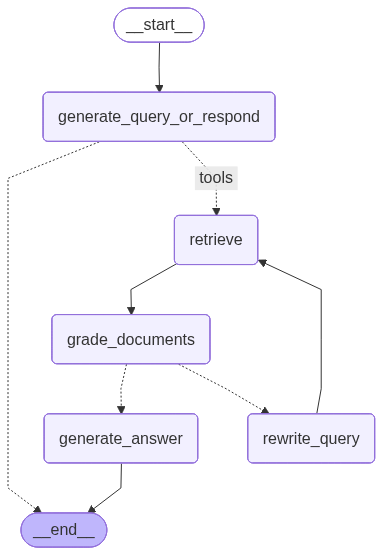
\includegraphics[width=0.65\textwidth]{agentic_rag_workflow.png}
    \caption{نمونه‌ای از گردش کار استنتاج هوشمند \lr{RAG}. این تصویر مراحل مختلف فرایند استنتاج را نشان می‌دهد، از جمله دریافت پرس‌وجو، تصمیم‌گیری برای بازیابی اسناد، و تولید پاسخ نهایی.}
    \label{fig:agentic_rag_workflow}
\end{figure}

\subsection{مراحل فرایند}
سیستم استنتاج هوشمند \lr{RAG} دارای گردش کار مبتنی بر گراف است که شامل مراحل زیر می‌باشد:

\subsection*{گره‌های اصلی}
\begin{itemize}
    \item \textbf{گره عامل (\lr{Agent Node}):} تصمیم‌گیری برای بازیابی اسناد یا پاسخ مستقیم
    \item \textbf{ابزار بازیابی (\lr{Retrieval Tool}):} جستجو برای اسناد مرتبط با استفاده از جستجوی ترکیبی
    \item \textbf{ارزیابی اسناد (\lr{Document Grading}):} بررسی میزان مرتبط بودن اسناد بازیابی شده
    \item \textbf{بازنویسی سؤال (\lr{Question Rewriting}):} بهبود سؤالاتی که نتایج مرتبط ارائه نمی‌دهند
    \item \textbf{تولید پاسخ (\lr{Answer Generation}):} تولید پاسخ نهایی با استفاده از بافت بازیابی شده
\end{itemize}

\subsection*{الگوریتم گردش کار}
فرایند تصمیم‌گیری سیستم به صورت زیر عمل می‌کند:

\begin{enumerate}
    \item \textbf{دریافت پرس‌وجوی کاربر:} سیستم پیام کاربر را دریافت و تحلیل می‌کند
    \item \textbf{تصمیم‌گیری اولیه:} عامل تصمیم می‌گیرد که آیا نیاز به بازیابی اسناد است یا می‌تواند مستقیماً پاسخ دهد
    \item \textbf{بازیابی شرطی:} در صورت نیاز، ابزار بازیابی فعال شده و اسناد مرتبط جستجو می‌شوند
    \item \textbf{ارزیابی کیفیت:} میزان مرتبط بودن اسناد بازیابی شده با پرس‌وجو ارزیابی می‌شود
    \item \textbf{حلقه بازخورد:} در صورت عدم مرتبط بودن، سؤال بازنویسی شده و فرایند تکرار می‌شود
\end{enumerate}


\subsection{فرایند تولید پاسخ}

\subsubsection*{حاشیه‌نویسی شناسه‌های بخش}
بخش‌های بازیابی شده به همراه شناسه‌های یکتای خود (\lr{chunk\_id}) به مدل زبان بزرگ ارسال می‌شوند. هر بخش با فرمت زیر حاشیه‌نویسی می‌شود(شکل \ref{fig:tool_response}).

این حاشیه‌نویسی به مدل زبان بزرگ اجازه می‌دهد تا دقیقاً مشخص کند کدام بخش‌ها در تولید پاسخ استفاده شده‌اند.

\begin{figure}[!htbp]
    \centering
    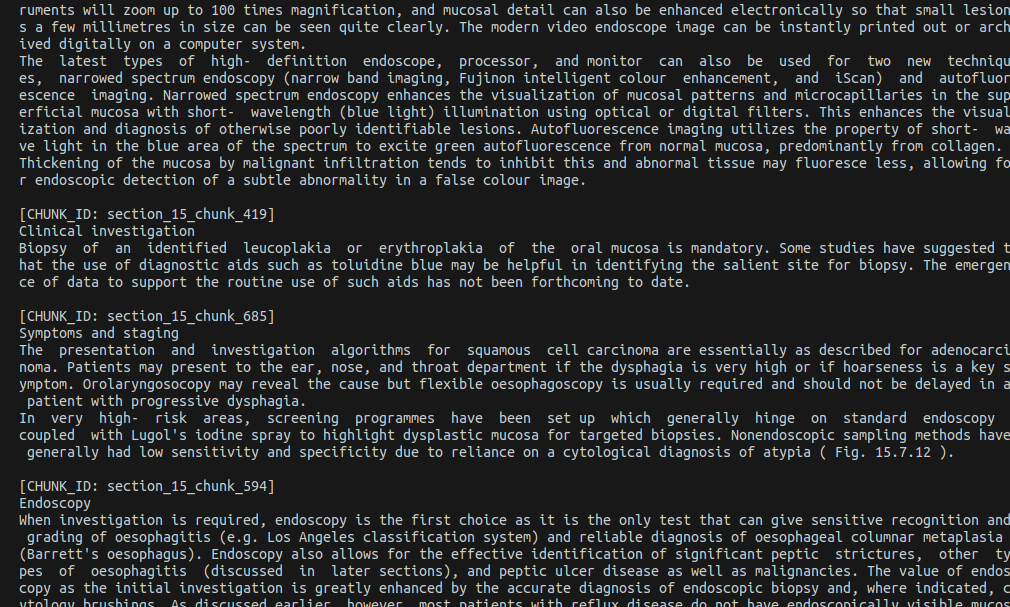
\includegraphics[width=0.95\textwidth]{tool_response.png}
    \caption{نمونه‌ای از پاسخ ابزار بازیابی که شامل بخش‌های حاشیه‌نویسی شده با شناسه‌های یکتا می‌باشد. این فرمت به مدل زبان بزرگ کمک می‌کند تا منابع استفاده شده را به دقت مشخص کند.}
    \label{fig:tool_response}
\end{figure}

\subsubsection*{تولید پاسخ ساختاریافته}
مدل زبان بزرگ پاسخی ساختاریافته تولید می‌کند که شامل دو بخش است:

\begin{itemize}
    \item \textbf{پاسخ (\lr{answer}):} متن پاسخ نهایی برای کاربر
    \item \textbf{شناسه‌های استفاده شده (\lr{chunk\_ids\_used}):} فهرست شناسه‌های بخش‌هایی که در تولید پاسخ مورد استفاده قرار گرفته‌اند
\end{itemize}

\noindent
نمونه‌ای از پاسخ ساختاریافته تولید شده توسط مدل:

\begin{latin}
\begin{verbatim}
{
  "answer": "Narrow band imaging, a type of narrowed 
  spectrum endoscopy, uses short-wavelength (blue light) 
  illumination with optical or digital filters. This 
  technique enhances the visualization of mucosal 
  patterns and microcapillaries in the superficial 
  mucosa, which helps in better visualizing and 
  diagnosing otherwise poorly identifiable lesions, 
  including distinguishing columnar from squamous mucosa.",
  "chunk_ids_used": [
    "section_15_chunk_101", 
    "section_15_chunk_620"
  ]
}
\end{verbatim}
\end{latin}

این ساختار به سیستم اجازه می‌دهد تا دقیقاً بخش‌های استفاده شده را شناسایی و متادیتای مرتبط را استخراج کند.

\subsection{استخراج متادیتا و بازیابی تصاویر}
پس از دریافت پاسخ از مدل زبان بزرگ، سیستم فرایند استخراج تصاویر مرتبط را آغاز می‌کند:

\subsubsection*{الگوریتم استخراج تصاویر}
\begin{enumerate}
    \item \textbf{شناسایی بخش‌های استفاده شده:} بر اساس \lr{chunk\_ids\_used}، اشیاء دقیق بخش‌ها از لیست بازیابی شده انتخاب می‌شوند
    \item \textbf{بررسی متادیتا:} برای هر بخش، فیلد \lr{meta.doc\_items} در متادیتا بررسی می‌شود
    \item \textbf{شناسایی تصاویر والد:} عناصری با برچسب \lr{"label": "picture"} شناسایی می‌شوند
    \item \textbf{استخراج شناسه تصویر:} از فیلد \lr{self\_ref} شناسه تصویر استخراج می‌شود
    \item \textbf{بازیابی تصویر کامل:} تصویر کامل به همراه توضیحات تولید شده توسط مدل چندوجهی از مخزن اسناد بازیابی می‌شود
    \item \textbf{الحاق به پاسخ:} تصاویر به پاسخ نهایی عامل الحاق می‌شوند
\end{enumerate}

این فرایند تضمین می‌کند که تمامی اطلاعات بصری مرتبط با پاسخ، به همراه متن، در اختیار کاربر قرار گیرد.

\subsection{پیاده‌سازی لایه رابط کاربری}
در لایه \lr{Framework}، یک ربات تلگرام پیاده‌سازی شده است که رابط کاربری تعاملی برای سیستم فراهم می‌آورد:

\subsubsection*{مدیریت بخش‌ها در ربات تلگرام}
\begin{enumerate}
    \item \textbf{ذخیره‌سازی بخش‌ها:} پس از دریافت پاسخ از عامل، بخش‌های استفاده شده در حافظه موقت ذخیره می‌شوند
    \item \textbf{تولید دکمه‌های تعاملی:} برای هر \lr{chunk\_id}، یک دکمه \lr{Inline Keyboard} در پیام تلگرام ایجاد می‌شود
    \item \textbf{پردازش کلیک کاربر:} هنگامی که کاربر روی دکمه شناسه بخش کلیک می‌کند، سیستم محتوای کامل بخش را از حافظه می‌خواند
    \item \textbf{نمایش جزئیات:} محتوای بخش به همراه متادیتای مرتبط برای کاربر نمایش داده می‌شود
\end{enumerate}

این رویکرد به کاربران اجازه می‌دهد تا شفافیت کاملی نسبت به منابع استفاده شده در تولید پاسخ داشته باشند و در صورت نیاز، محتوای اصلی بخش‌ها را مشاهده کنند.

\section{نتیجه‌گیری}
سیستم استنتاج هوشمند \lr{RAG} با استفاده از \lr{LangGraph} قابلیت‌های پیشرفته‌ای برای تصمیم‌گیری خودکار و بهینه‌سازی فرایند بازیابی اطلاعات فراهم می‌آورد. این رویکرد نه تنها کارایی سیستم را بهبود می‌بخشد بلکه تجربه کاربری بهتری نیز ارائه می‌دهد. ترکیب تصمیم‌گیری هوشمند، ارزیابی کیفیت اسناد، و بازنویسی پرس‌وجو منجر به سیستمی قدرتمند و انطباق‌پذیر شده است که می‌تواند در کاربردهای مختلف پردازش اسناد پزشکی مورد استفاده قرار گیرد.

% ------- References Page -------
\newpage
\LTRSection{References}
\begin{thebibliography}{10}
    \bibitem[1]{ref-1} C. Ribeiro, “Sports scheduling: Problems and applications,” International Transactions in Operational Research, vol.19, pp.201–226, Jan. 2012.
\end{thebibliography}
\end{document}